% ============================================================
% ปกหน้าตำราวิชาการ (Academic Book Cover)
% มาตรฐาน มหาวิทยาลัยราชภัฏรำไพพรรณี
% ============================================================
\thispagestyle{empty}
\begin{titlepage}
\begin{tikzpicture}[remember picture, overlay]
    % พื้นหลังหลักไล่ระดับสีน้ำเงินราชภัฏ
    \fill[left color=rbruNavy!98!black, right color=rbruNavy!88!agriForest] 
        (current page.south west) rectangle (current page.north east);
    
    % แถบขลิบทองราชภัฏแนวตั้งทางซ้าย
    \fill[color=rbruGold] 
        ([xshift=2.4cm]current page.south west) rectangle ([xshift=2.6cm]current page.north west);

    % เส้นเรขาคณิตเวกเตอร์ฟิสิกส์คณิตศาสตร์โปร่งแสง
    \draw[color=white, opacity=0.08, line width=1.0pt]
        ([xshift=3.5cm, yshift=-2.5cm]current page.north west) -- ([xshift=-1.5cm, yshift=5cm]current page.south east);
    \draw[color=rbruGold, opacity=0.12, line width=1.2pt]
        ([xshift=3.5cm, yshift=-6cm]current page.north west) -- ([xshift=-1cm, yshift=2cm]current page.south east);

    % ข้อมูลสังกัดด้านบน
    \node[anchor=north west, text width=14.5cm] at ([xshift=3.2cm, yshift=-2.0cm]current page.north west) {
        {\fontsize{14}{18}\selectfont\bfseries\color{rbruGold} คณะวิทยาศาสตร์และเทคโนโลยี มหาวิทยาลัยราชภัฏรำไพพรรณี\par}
        \vspace{2pt}
        {\fontsize{10}{13}\selectfont\color{softMist!85} โครงการพัฒนาทักษะวิชาชีพชั้นสูงเพื่อการขับเคลื่อนเศรษฐกิจฐานนวัตกรรม (AIoT 2570)\par}
    };

    % ส่วนชื่อเรื่องหลัก (Main Title Block)
    \node[anchor=north west, text width=15.2cm] at ([xshift=3.2cm, yshift=-3.4cm]current page.north west) {
        {\color{rbruGold}\rule{0.45\textwidth}{3pt}\par}
        \vspace{8pt}
        {\fontsize{28}{35}\selectfont\bfseries\color{white} หลักสูตรเกษตรดิจิทัล\par}
        \vspace{3pt}
        {\fontsize{26}{33}\selectfont\bfseries\color{white} และปัญญาประดิษฐ์ฝังตัว\par}
        \vspace{7pt}
        {\fontsize{15}{21}\selectfont\bfseries\color{durianGold} สวนผลไม้มูลค่าสูงและการเพาะเลี้ยงสัตว์น้ำชายฝั่ง ภาคตะวันออก\par}
        \vspace{5pt}
        {\fontsize{9}{13}\selectfont\color{softMist!85} Digital Agriculture and Embedded Artificial Intelligence Curriculum\\for High-Value Fruit Orchards and Coastal Aquaculture\par}
        \vspace{8pt}
        {\color{rbruGold}\rule{0.75\textwidth}{1.2pt}\par}
    };

    % กรอบภาพศิลป์ปก Masterclass (Cover Artwork Window)
    \node[anchor=center, draw=rbruGold, line width=2.0pt, rounded corners=6pt, inner sep=0pt, fill=black] 
        at ([xshift=1.0cm, yshift=-1.0cm]current page.center) {
        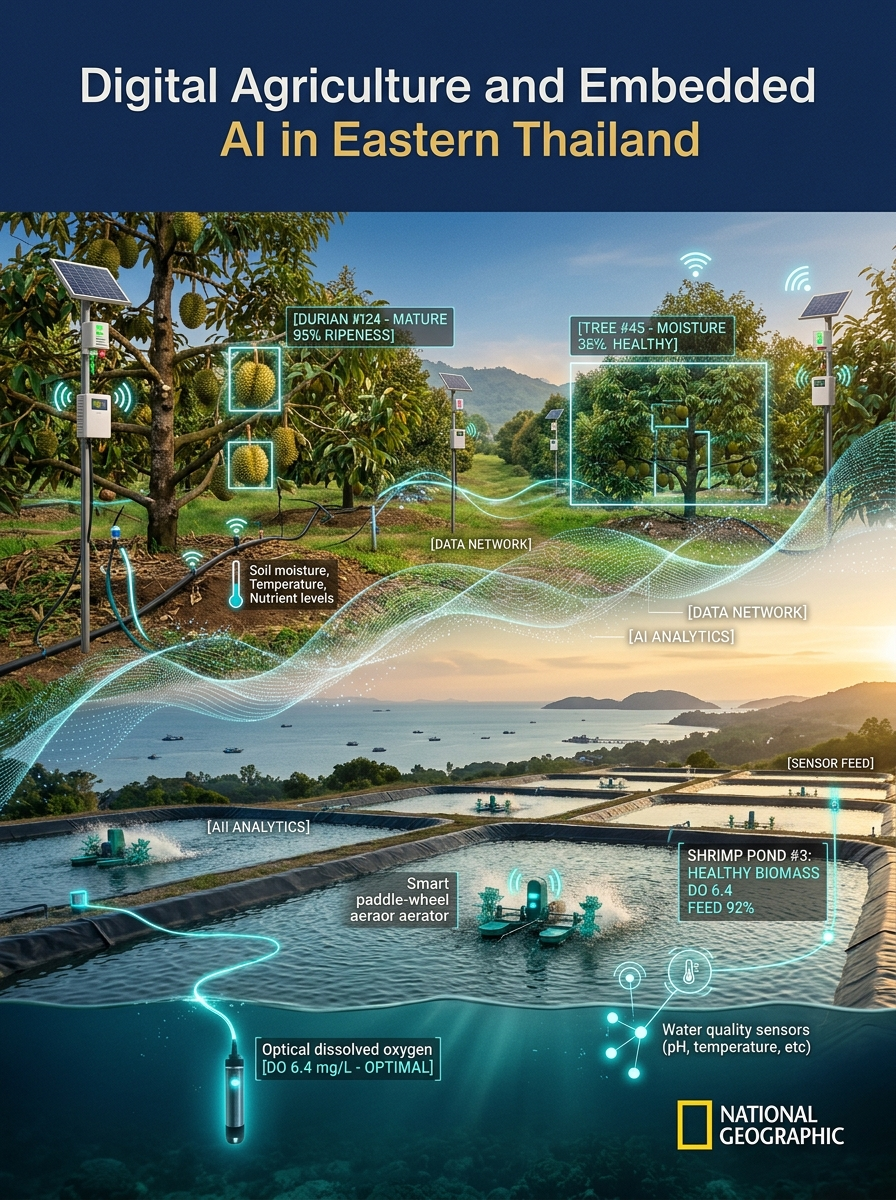
\includegraphics[width=14.5cm, height=9.2cm, keepaspectratio=false]{figures/cover_artwork.jpg}
    };

    % รายนามคณะผู้เขียนและสำนักพิมพ์ด้านล่าง
    \node[anchor=south west, text width=14.5cm] at ([xshift=3.2cm, yshift=1.8cm]current page.south west) {
        {\fontsize{12}{15}\selectfont\bfseries\color{white} ผู้ช่วยศาสตราจารย์ ดร.ชีวะ ทัศนา\par}
        \vspace{2pt}
        {\fontsize{9.5}{12}\selectfont\color{softMist!90} ร่วมกับคณะวิทยากรผู้ทรงคุณวุฒิ คณะวิทยาศาสตร์และเทคโนโลยี\par}
        \vspace{2pt}
        {\fontsize{8.5}{11}\selectfont\color{softMist!75} ผศ.อรรถกร คำฉัตร \textbar\ ผศ.ดร.ณมนรัก คำฉัตร \textbar\ รศ.ดร.นิภัทร เปี่ยมอรุณ \textbar\ ผศ.ดร.จิรภัทร จันทมาลี\par}
        {\fontsize{8.5}{11}\selectfont\color{softMist!75} ผศ.นิคม รัตนโรจนกุล \textbar\ รศ.ดร.นันทพร มูลรังษี \textbar\ ผศ.ดร.สุพัตรา รักษาพรต\par}
        \vspace{10pt}
        {\color{rbruGold}\rule{0.35\textwidth}{0.8pt}\par}
        \vspace{4pt}
        {\fontsize{10}{13}\selectfont\bfseries\color{rbruGold} สำนักพิมพ์มหาวิทยาลัยราชภัฏรำไพพรรณี \quad \textbar \quad \color{softMist!80}พ.ศ. 2570\par}
    };
\end{tikzpicture}
\end{titlepage}
\clearpage
